%
% LaTeX template document for METIS Documentation
% 
% M. Kenworthy 2016 May 29
%
% vim: tw=80
%
\documentclass[a4paper,11pt]{article}

%%%%%%%%%%%%%%%%%%%%%%%%%%%%%%%%%%%%%%%%%%%%%%%%%%%%%%%%%%%%%%%
%%% PUT IN YOUR METIS DOCUMENT NUMBERS IN THE COMMANDS BELOW  %
%%%%%%%%%%%%%%%%%%%%%%%%%%%%%%%%%%%%%%%%%%%%%%%%%%%%%%%%%%%%%%%

\newcommand{\DocTitle}{VLT Pupil Geometry and HCI Pupil Masks}
\newcommand{\DocNum}{}
\newcommand{\DocIssue}{v2}
\newcommand{\IssueDate}{22 Jan 2018}
\newcommand{\Issue}{}

%%%%%%%%%%%%%%%%%%%%%%%%%%%%%%%%%%%%%%%%%%%%%%%%%%%%%%%%%%%%%%%%%%%%%%%%
%%% PACKAGES
%%%%%%%%%%%%%%%%%%%%%%%%%%%%%%%%%%%%%%%%%%%%%%%%%%%%%%%%%%%%%%%%%%%%%%%%

% setting the paper size
% guesstimated from Word Template
% footskip to make room for METIS logo in lower right
% headheight to make header not jump around the place
\usepackage[headheight=28pt]{geometry}
% debugging by drawing bounding boxes around major frames
%\usepackage[showframe]{geometry}
\geometry{textwidth=16cm,textheight=23.75cm,left=25mm,top=25mm,footskip=40pt}


% needed to get page x of y in footers
\usepackage{lastpage}

% quote filenames and URLs correctly
\usepackage[obeyspaces]{url}

% be able to put in graphics
\usepackage{graphicx}

% make vertical red lines in header and footer
\usepackage{colortbl}

% fancy headers and footers
\usepackage{fancyhdr}
% put header and footers on all pages except the cover page
\pagestyle{fancyplain}


\usepackage{color}
\definecolor{darkblue}{rgb}{0.0, 0.0, 0.5}


% add capability for clickable hyperlinks that will directly compile
% using pdflatex

\usepackage[backref,breaklinks,colorlinks=true,urlcolor=blue,citecolor=blue,linkcolor=darkblue,pdftitle={\DocTitle}, pdfauthor={Matthew A. Kenworthy}]{hyperref}

% top header on document
% tabular used to get vertical red lines
% sffamily puts it in Sans Serif
%\lhead{\renewcommand{\arraystretch}{2.0} \sffamily\begin{tabular}{ l !{\color{red}\vrule} l !{\color{red}\vrule} l !{\color{red}\vrule} l} \IssueDate & \DocTitle{} & \DocNum{} & \Issue{} \end{tabular} }
\lhead{\sffamily\begin{tabular}{p{7.2cm} p{4.4cm} p{0.8cm} p{3.0cm}
}\DocTitle{} & \DocNum{} & \Issue{} & \IssueDate{} \end{tabular} }
\chead{}
\rhead{}
\lfoot{}
\cfoot{\sffamily Page {\bf\sffamily \thepage}\ of {\bf\sffamily \pageref{LastPage}}}
% the METIS logo
%\rfoot{ \raisebox{-.5\height}{\includegraphics[width=3cm]{metis_ring.png}} }

\renewcommand{\headrule}{\hbox to\headwidth{%
  \color{red}\leaders\hrule height \headrulewidth\hfill}}

% remove header and footer lines
%\renewcommand{\headrulewidth}{0.0pt}
\renewcommand{\footrulewidth}{0.0pt}

% use titlesec to change the fonts of section headers and add red
% underline
\usepackage{titlesec}

\titleformat{\section}
  {\normalfont\Large\sffamily}{\thesection}{1em}{}[\titleline{\color{red}\titlerule[0.8pt]}]
\titleformat{\subsection}
  {\normalfont\large\sffamily}{\thesubsection}{1em}{}[]
\titleformat{\subsubsection}
  {\normalfont\large\sffamily}{\thesubsubsection}{1em}{}[]

% making good tables with no vertical lines - all horizontal
\usepackage{booktabs}

% more space between table rows using the command \ra
\newcommand{\ra}[1]{\renewcommand{\arraystretch}{#1}}

% the color package allows us to define non-standard colours in the latex output
\usepackage{color}
\definecolor{darkblue}{rgb}{0.0, 0.0, 0.4}

% we use the hyperref package so that our links are clickable in a PDF reader
\usepackage{hyperref}
\hypersetup{colorlinks=true,citecolor=darkblue,linkcolor=black}

% No ident on paragraphs and a line skip
\usepackage[parfill]{parskip}

% defs for bibtex files from arXiv.org
\def\apjl{ApJL }
\def\aj{AJ }
\def\apj{ApJ }
\def\pasp{PASP }
\def\spie{SPIE }
\def\apjs{ApJS }
\def\araa{ARAA }
\def\aap{A\&A }
\def\nat{Nature }

% set all tables to have a red border
\arrayrulecolor{red}
\ra{1.3}

\begin{document}

%%%%%%%%%%%%%%%%%%%%%%%%%%%%%%%%%%%%%%%%%%%%%%%%%%%%%%%%%%%%%%%%%%%%%%%%
%%% TITLE PAGE FOR REIS DOCUMENT
%%%%%%%%%%%%%%%%%%%%%%%%%%%%%%%%%%%%%%%%%%%%%%%%%%%%%%%%%%%%%%%%%%%%%%%%

\begin{titlepage}
%\includegraphics[width=0.40\textwidth]{metis_simple}\par\vspace{5cm}

\noindent\makebox[\linewidth]{\textcolor{red}{\rule{\columnwidth}{1pt}}}
\vspace{1cm}
\sffamily{\Huge \textsf{\DocTitle{}} \par}
\vspace{-1.2cm}
\noindent\makebox[\linewidth]{\textcolor{red}{\rule{\columnwidth}{1pt}}}

{\LARGE \DocNum{}\par}
{\LARGE \DocIssue{}\par}
{\LARGE \IssueDate{}\par}

\vfill

% Bottom of the page
\begin{table*}[ht]
\centering
\begin{tabular}{@{} *{4}{p{3.5cm}} @{}}\toprule
%\begin{tabular}{@{}p{3.5cm} p{3.5cm} p{3.5cm} p{3.5cm} @{}}\toprule
          & \small Signature and approval &  &  \\ \midrule
          & \small Name              & \small Date       & \small Signature \\
\midrule
Prepared: & M. Kenworthy and D.S. Doelman & 22.01.2018 &           \\
Checked:  &                   &            &           \\
Approved: &                   &            &           \\
\bottomrule
\end{tabular}
\end{table*}

\end{titlepage}

%\clearpage

\section*{Revision History}

\begin{tabular}{l l l l}\toprule
Issue  	& Date 		& Section/Page affected & Reason/Remarks \\ \midrule
v2 	& 22.01.2018 	& All 			& Converted from Google Doc \\
\bottomrule
\end{tabular}

\clearpage
\tableofcontents

%\clearpage
\listoffigures

%\clearpage
\listoftables

\clearpage

\section{Introduction}

\subsection{Scope}

\subsection{Applicable and Reference Documents}

\begin{tabular}{@{}lp{6cm}lll@{}}
\toprule
RD 	& Title 							& Reference & Issue & Date \\
\midrule
RD1	& Shape of Cassegrain Pupil at VLT-UT4      			& ERIS Memo OAA-17-001		&2       & 07/07/2017  \\
	RD2	& ERIS-NIX Pupil Masks Requirements Specification v1.0      	& VLT-SPE-ERI-14402-2009	&1.0     & 07/04/2017  \\
RD3	& VLT optical prescription for the ERIS focal station       	& VLT-TRE-ERI-14401-3103	&1.0	&  23/03/2017  \\
RD4	& M2-spiders general assembly     				& VLT-DWG-AES-11310		&	&  15/01/1994 \\
\bottomrule
\end{tabular}

\subsection{Abbreviations and Acronyms}

\begin{tabular}{@{}ll@{}}
\toprule
Acronym & Definition \\
\midrule
ESO     & European Southern Observatory \\
VC      & Vortex Coronagraph           \\
RAVC    & Ring Apodized Vortex Coronagraph \\
APP     & Apodizing Phase Plate        \\
AGPM    & Annular Grooved Phase Mask   \\
CFO2    & Common Fore Optics Version 2 \\
\bottomrule
\end{tabular}

\clearpage

\section{Introduction}
Two pupil masks are required for ERIS coronagraphy - a mask for the APP180 and
a Lyot mask for the Vortex coronagraph. Both masks are not in the reimaged
pupil plane of ERIS, but are a distance of $4.40mm$ out of this plane.

The APP-180 requires a pupil mask to ensure that only light from the pupil
enters the APP coronagraph optic. The steps needed to determine this are
detailed in RD2. After this document was released, it was noted that a pupil
image from VISIR shows warm thermal emission from not only the secondary mirror
and its supports, but also a surrounding light baffle on M2, and from M3 when
it is fixed in its stow position - this was detailed in RD1.

We combine the results from these documents into this document to provide a
single reference for the justification we have on the masks and provide a
Python computer code that generates a binary mask that masks out the warm
optical elements in the VLT optical beam.


\section{The Geometry of the VLT Pupil}

An engineering drawing from the VLT shows the location of the secondary support structures and the secondary hub with respect to the optical centre of the mirror. There are a list of critical radii concerned with determining the VLT UT4 pupil listed in Table 1.




\begin{table}[h]

\begin{tabular}{@{}p{1cm} p{7cm} l p{5cm}@{}}
\toprule
Radius (mm)& Relevant optical component & Reference & Notes \\
\midrule
4219.7 & Secondary support crossing coordinate system of primary mirror in drawings & RD4 & Used for fixing where the spider arm crosses the axes \\
4092 & M1 radius & RD4 & David Henry email to MAK 12/1/2018 \\
4060 & ERIS Entrance Pupil (M2 projected onto M1) & RD3 & Confirmed David Henry email to MAK 12/1/2018 \\
775 & M2 sky baffle & & \\
646.5 & DSM wind screen external diameter on UT4 & RD1 & Screen is emissive and needs blocking \\
558 & M2 mirror diameter & & \\
\bottomrule
\end{tabular}
\caption{ \label{tab:tablesadf} Relevant radii of optical components in ERIS and the VLT.}
\end{table}


We define a coordinate system centred on the middle of the primary mirror. The
spider arms are tilted at an angle of 5.5 degrees with respect to the axes of
this coordinate system, and they all cross at a radius of 4219.7mm. The Python
code used to generate the pupil masks defines a square image whose size equals
2 times 4219.7mm, marking the point where the spiders cross the coordinate axes
of the primary mirror as at the midpoint of each side of the square.

The radius of the primary is at 4092mm.

ERIS follows the design of many IR instruments and so the mirror M2 is
undersized with respect to M1, and the projected radius of M2 is 558mm, which
when reprojected onto M1 is a diameter of 4060mm.

The diameter of 4060mm is the defined pupil of ERIS, and this dimension is used
in simulations and raytracing through to the location of the pupil in ERIS.

\section{The geometry of the ERIS pupil}

The L/M camera optics in ERIS are referred to as 'Camera 3' with a 13mas/pix
scale at the camera focal plane. This is a large oversampling of the PSF but it
is necessary due to the large sky background in ERIS and is required to prevent
saturation of the detector.

The optics are refractive lenses, and so the image of the pupil formed at the
location of the coronagraphs is blurred by a few tens of microns. To ensure all
light from the pupil and no light from thermal emission of nearby warm
telescope components, the pupil is undersized for two effects - the reimaging
out of pupil plane of the pupil, and for the alignment and flexure budget of
ERIS.

Two movable wheels are on either side of the pupil location in ERIS (see
Figure~\ref{fig:wheels}). In this figure, light from the
telescope comes from the {\bf right}, passes through a tilted filter, then the Pupil
plane has a fixed cold aperture of 13mm in place, and then the pupil wheel
where the gvAPP optic will be located.

\begin{figure}[htp]
\centering
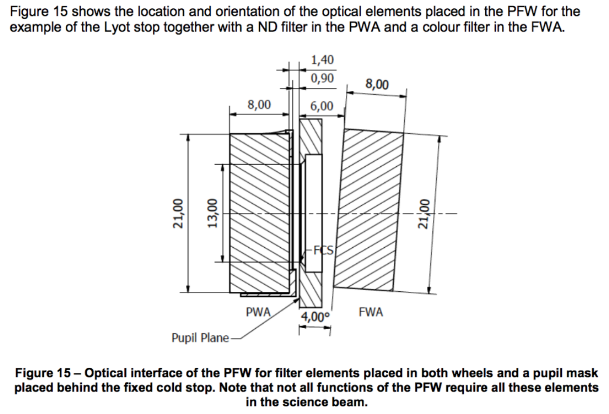
\includegraphics[angle=0,width=\columnwidth]{optical_interface}
\caption{ \label{fig:wheels} Optical interface of the PFW. Figure from
R2.}
\end{figure}

The geometry of the gvAPP for ERIS is shown in Figure~\ref{fig:gvapp} - sent by Jason
Kekas in 2018 Jan 18 email. Matt K local link

\begin{figure}[htp]
\centering
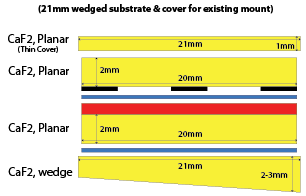
\includegraphics[angle=0,width=0.7\columnwidth]{21mmOption_with_cover-02}
\caption{ \label{fig:gvapp} Assembly diagram of the gvAPP for ERIS.}
\end{figure}

\section{Size of the pupil in the pupil plane}

The image of the outer edge in the pupil plane is not a sharp transition, but
goes from 100 to 0 percent transmission from 5.8mm to 6.3mm. We define the
radius of the pupil image in ERIS Camera 3 to be 6.025mm, by visual inspection
of Figure 5 of RD2 for the half power point of the L band curves (see
Figure~\ref{fig:radpup}).

\begin{figure}[htp]
\centering
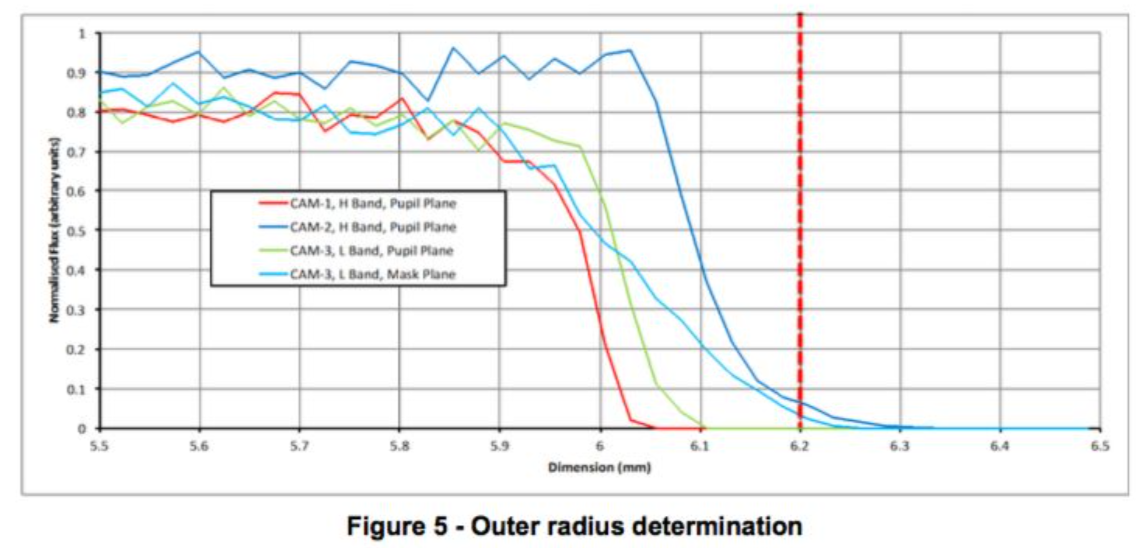
\includegraphics[angle=0,width=0.7\columnwidth]{pupil_cut}
\caption{ \label{fig:radpup} Figure 5 from RD2 showing a radial cut
through the raytraced image.}
\end{figure}

The 6.025mm was checked in ZEMAX and found to be 6.009mm. The 6.025mm number
was kept for the rest of the calculations.  Size of the pupil in the plane of
the gvAPP pattern There are three effects that reduce the effective area of the
illuminated pupil. First is the mechanical and alignment tolerances within ERIS
and the VLT. The second is the blurring due to the optical train, and the
change in pupil position as a function of field position because the optic is
no longer at the pupil plane. The third is that the pupil plane is in a
converging beam, and so the pupil image becomes smaller out of the pupil plane.

The distance from pupil plane in ERIS to the gvAPP pattern is 1.40mm from the
pupil plane to the mechanical interface, and 3.00mm from the gvAPP surface to
the gvAPP pattern, meaning that there is d=4.40mm from the ERIS pupil plane to
the gvAPP pattern, all in a converging beam.

A ZEMAX file with the details of the ERIS optical design called ERIS-NIX
205.zar from David Henry on 2018 Jan 17 (Matt K local link) was used to
calculate the size and blurring effects of the pupil.


\subsection{Demagnification of the pupil}

The pupil scales down by 0.977427 from 6.025mm to 5.89mm at the location of
d=4.40mm behind the ERIS pupil, and these calculations are detailed in a
spreadsheet. (From David Doelman on 18 Jan 2018: a spreadsheet detailing the
pupil image geometry % \texttt{ERIS_Pupil_alignment_tolerances.xlsx} 

\subsection{Pupil movement as a function of field position}

The gvAPP is not in the pupil plane, so there is a lateral shift of the pupil image for different field positions. The gvAPP is used in a beamswitching capacity, between two positions that are 5 arcseconds either side of the centre of the field of view. These calculations are detailed in the spreadsheet above, and this leads to a reduction of the pupil structures by 110 microns.

\subsection{Tolerances of ERIS alignment}

There is an additional amount of uncertainty in the location of the ERIS
pupil image in the pupil wheel, due to flexure and reattachment
tolerances in the design, estimated in Table~\ref{tab:errors}. This adds another 154 microns of blurring to the resultant pupil mask.

\begin{figure}[htp]
\centering
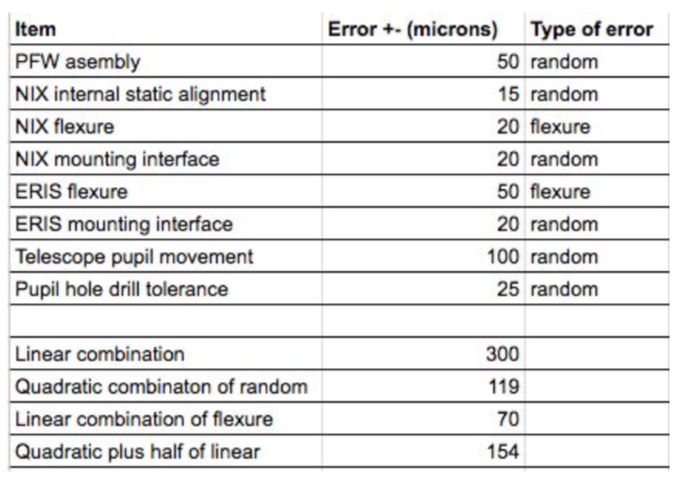
\includegraphics[angle=0,width=0.7\columnwidth]{error_budget}
\caption{ \label{tab:errors} Contributions to the error budget in the
location of the telescope pupil in ERIS.}
\end{figure}

\section{Additional warm structures in the VLT pupil}

The thermal infrared image of UT4 as taken by VISIR shows the presence of the stowed M3 mirror and a wind baffle at M2.

The Deformable Secondary Mirror will replace M2 in the future, and its diameter is listed in the table above. The M3 mirror in stow can be masked with the addition of a rectangular mask extending out to one side of the M2 circular obstruction.

The width of the spider arms are 40mm.

Light from the sky can go past the side barrel of M2 and go directly
into wide field visible wavelength instruments, adding to the sky
background. This is an issue for instruments such as MUSE, and to
prevent this direct line of sight propagation, a sky baffle is added
around the barrel of M2. This baffle is uncooled, and appears as a warm
emissive surface in the field of view of ERIS at thermal wavelengths.

The radius of this baffle is 775mm.

An overlay of the pupil generated in A is shown overlaid on the VLT
VISIR pupil image in Figure~\ref{fig:visir}. It can be seen that the
ERIS pupil matches the secondary support structure, the M3 baffle and
the expected radius of the M2 sky baffle.

\begin{figure}[htp]
\centering
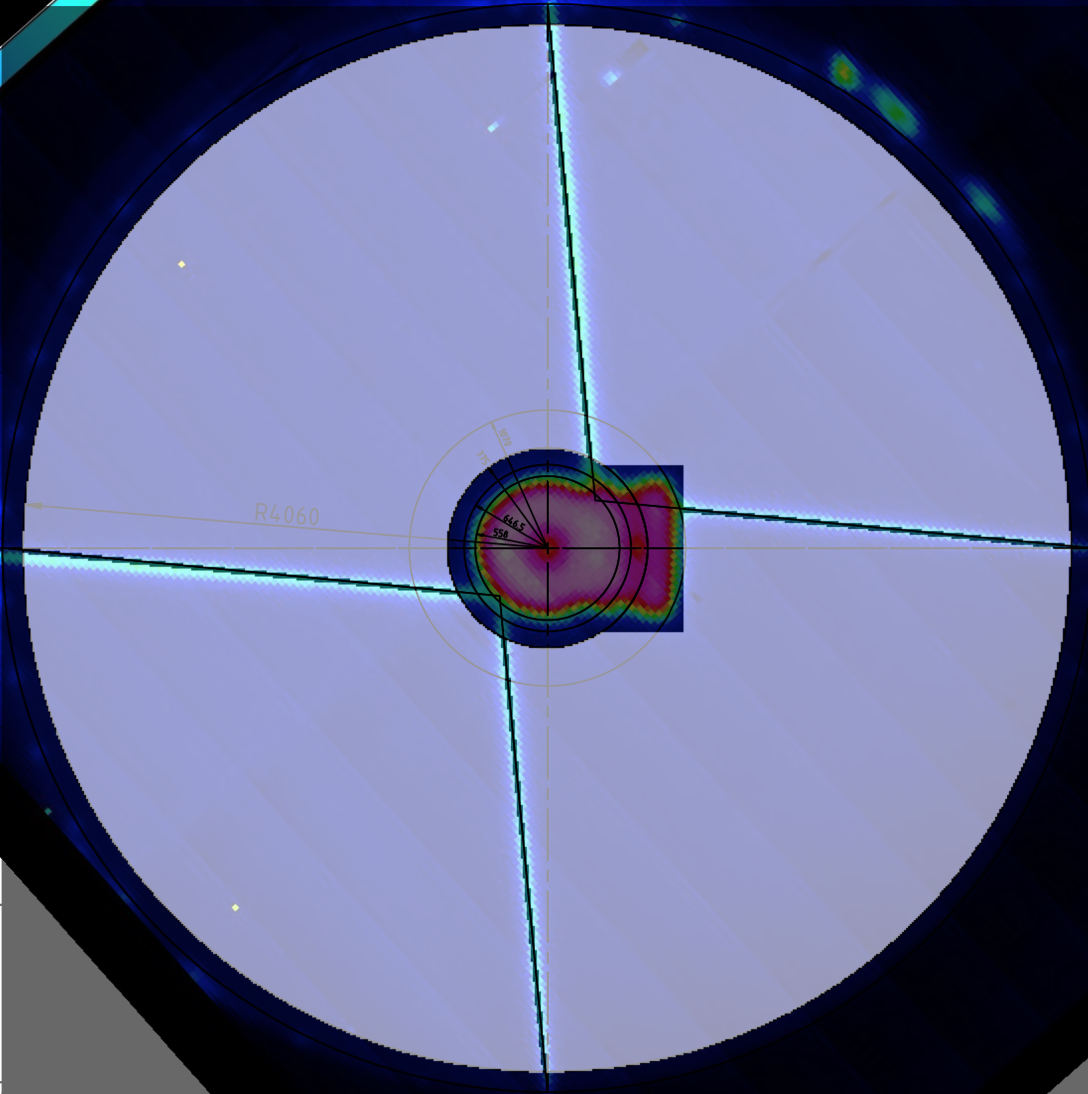
\includegraphics[angle=0,width=0.7\columnwidth]{vlt_visir_pupil}
\caption{ \label{fig:visir} The VLT UT4 pupil as seen by VISIR.}
\end{figure}

\section{Code to generate the gvAPP pupils}

The Python code \url{ERIS_pupil_tight_ZEMAX_corrected_SkyBaffle.py}
generates three pupil masks based on the discussions above. They are
labelled \url{VLT_ERIS_pupil_X_*.fits} ...where X is a letter A, B, or
D described in Table~\ref{tab:programs}. We use D for the design of
the gvAPP ERIS pupil. The code produces the masks with a pixel size of 5
microns. The demagnification is currently hard-coded in the pixel size
in the code, so it is inconsistent with the real pixel size. The box and
sky baffle are slightly demagnified but the kernel convolution
overwhelms this demagnification factor.



\begin{table}[h]
\begin{tabular}{@{}p{5cm}p{10cm}@{}}
\toprule
Pupil mask & Comment \\
\midrule
	\url{VLT_ERIS_pupil_A_entrance_pupil_SkyBaffle} & A is the with the sky baffle but no blurring at all at d=4.40mm plane with CaF2 substrate for a thickness of 3.00mm. \\
	\url{VLT_ERIS_pupil_B_undersized_out_of_pupil_plane_SkyBaffle} & B is blurred by the kernel for out of pupil plane field dependencies with +/- 5 arcsec field of view (110 microns total kernel size). \\
	\url{VLT_ERIS_pupil_D_tightly_undersized_ZEMAX_corrected_SkyBaffle} & D is convolved with an additional 154 micron kernel for the flexure and combination of alignment tolerances. This is the mask that should be used. \\
\bottomrule
\end{tabular}
\caption{\label{tab:programs} Python script names and the description of the
pupils they produce.}
\end{table}

\section{Orientation of mask with respect to the optical path}

The addition of the M3 baffle to mask out the M3 baffle means that the
symmetry of the mask is broken, and the orientation with respect to the
gvAPP glass subtrates needs to be determined.
%
We use a ZEMAX drawing of ERIS optics with Camera 3 in the beam, and
photos of UT4 to derive the orientation of the masks in
Figure~\ref{fig:eris}.
%
The python code generates the pupil to be consistent with the VISIR
orientation and needs to be rotated by 90 degrees to match the
orientation of the chromium pupil mask shown below.

\begin{figure}[htp]
\centering
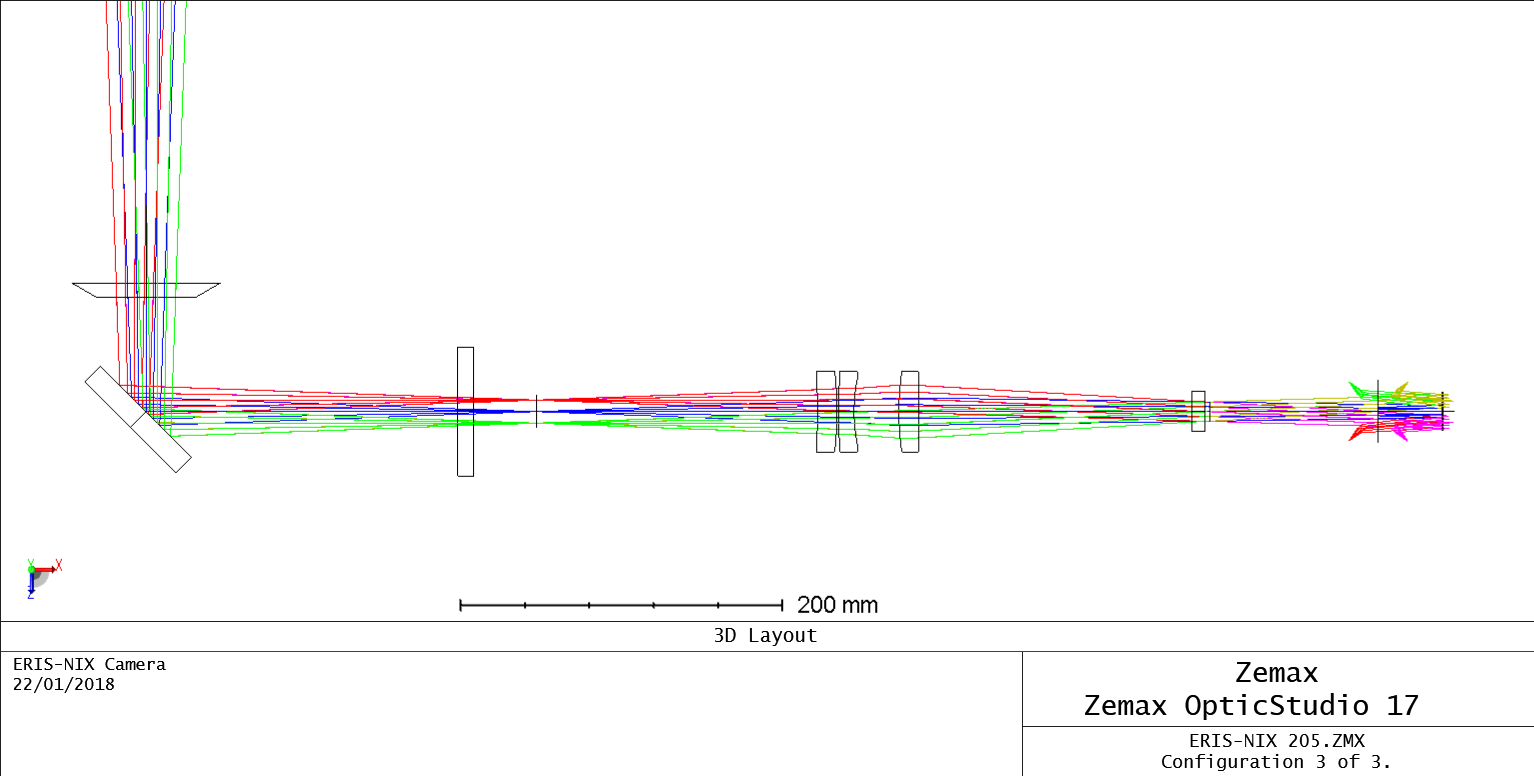
\includegraphics[angle=0,width=\columnwidth]{ERIS_Conf3_Layout}
\caption{ \label{fig:eris} The ERIS optical layout from the ZEMAX
file.}
\end{figure}

The appropriate configurations for the mask substrate and the liquid
crystal substrate are shown in Figure~\ref{fig:vltmap1} and \ref{fig:vltmap2}.

\begin{figure}[htp]
\centering
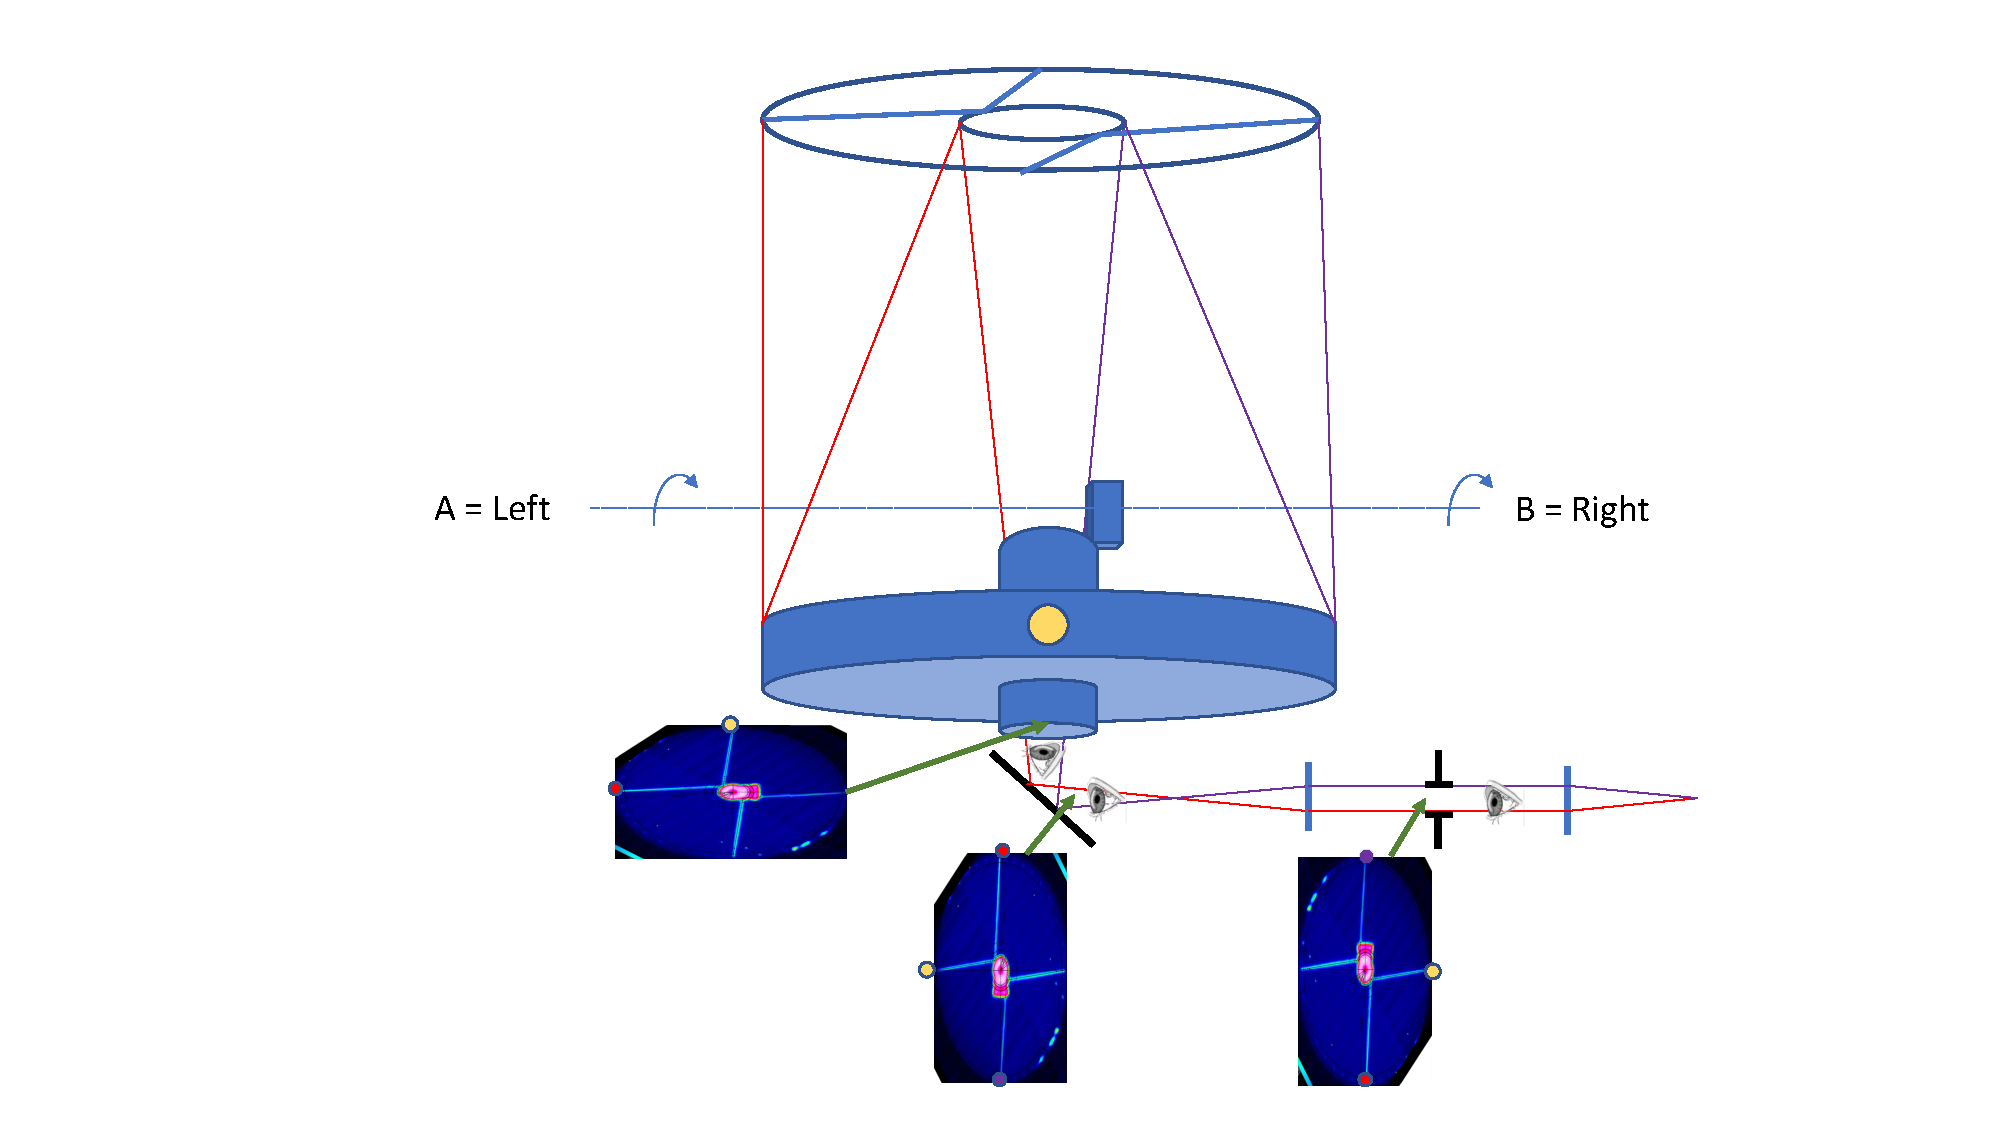
\includegraphics[angle=0,width=\columnwidth]{app_layout_p1}
\caption{ \label{fig:vltmap1} The optical path of VLT and ERIS
showing the relative orientation of the UT4 pupil with respect to the
pupil wheel.}
\end{figure}

\begin{figure}[htp]
\centering
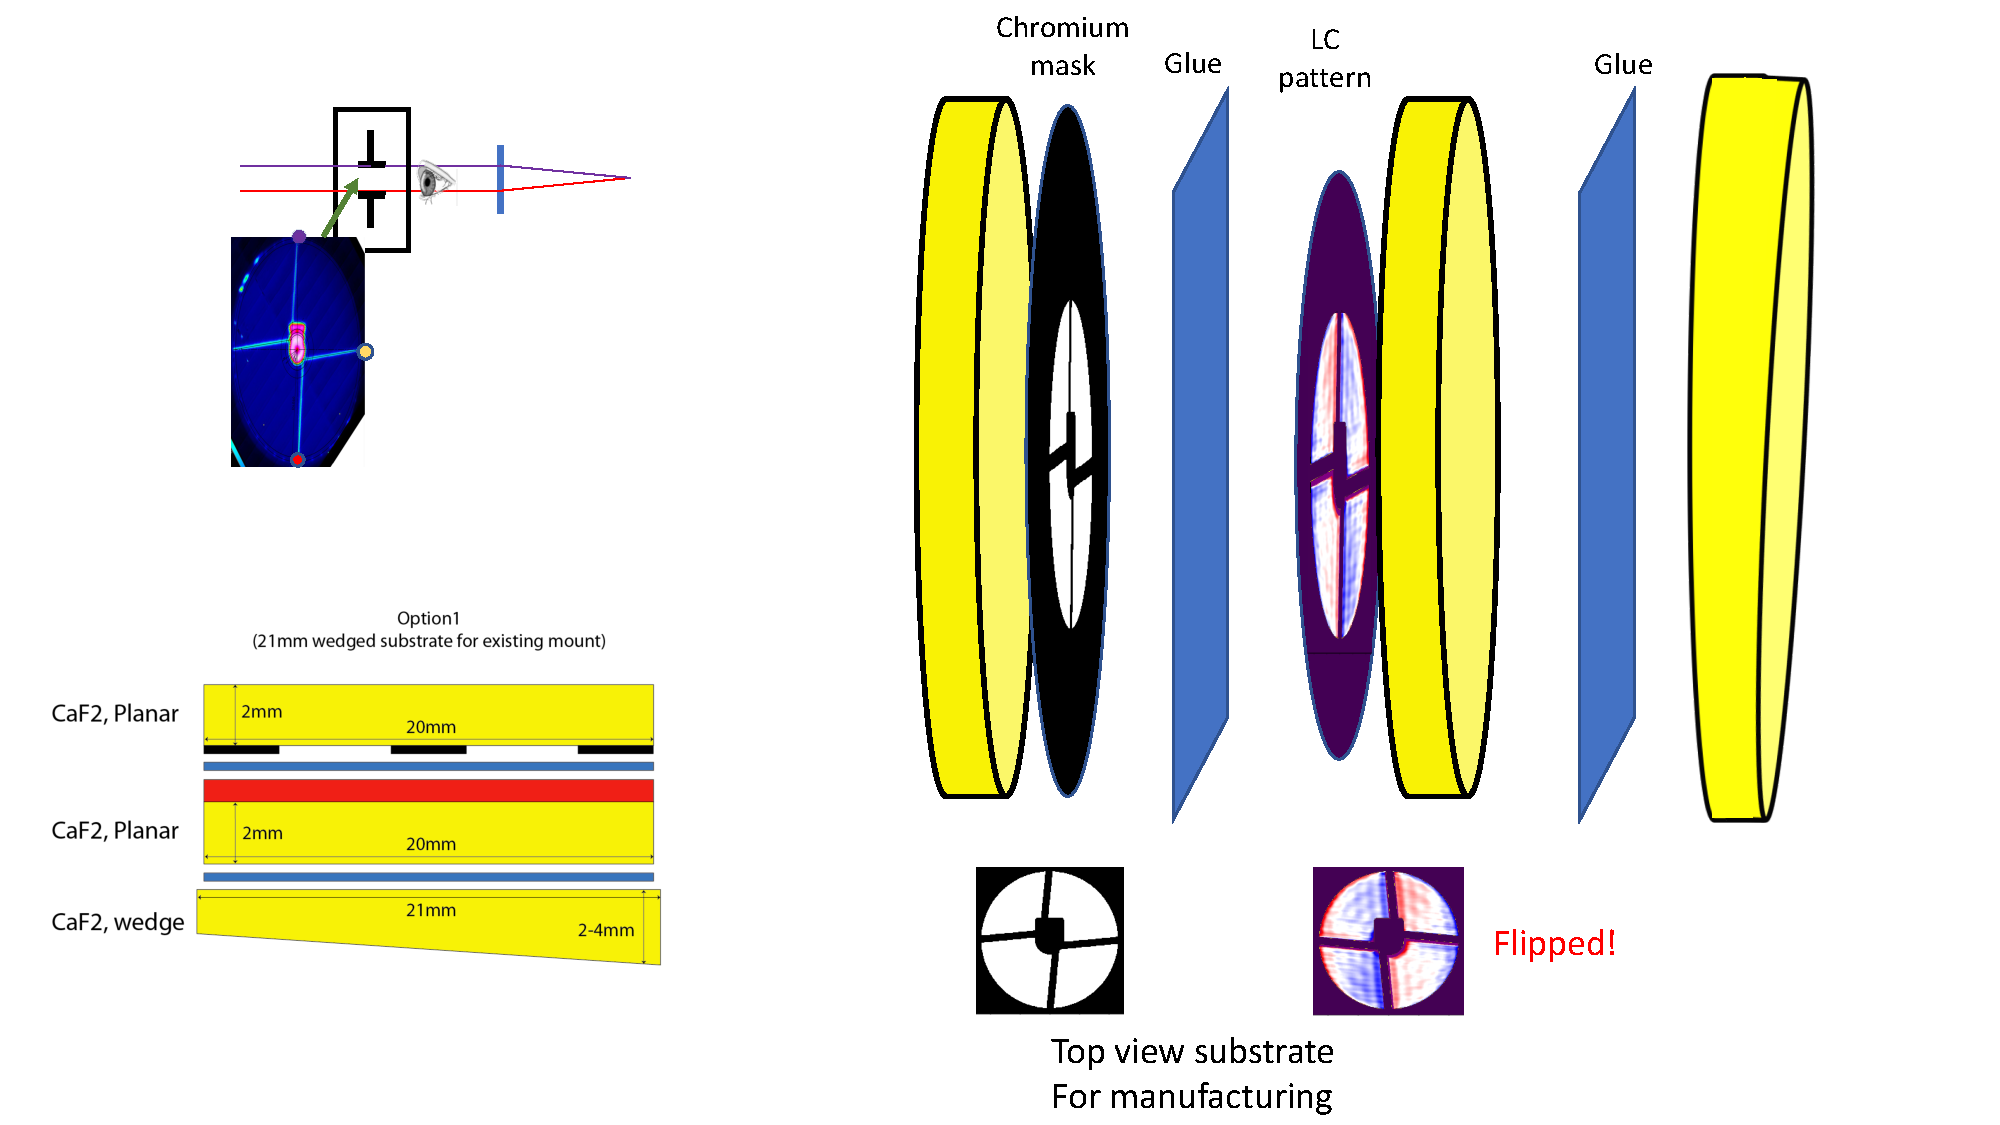
\includegraphics[angle=0,width=\columnwidth]{app_layout_p2}
\caption{ \label{fig:vltmap2} Detail of the optical path and assembly of
the gvAPP mask.}
\end{figure}


\bibliographystyle{nsf}
\bibliography{apj-jour,kenworthy}

% how to include graphics in your latex document
%\begin{figure}[htp]
%\centering
%\includegraphics[angle=270,scale=0.8]{simple_graph}
%\caption{ \label{graph1} A simple graphic built into the latex document.  }
%\end{figure}

\centering
END OF DOCUMENT

\end{document}

